\documentclass[a4paper]{scrartcl}
\usepackage[ngerman]{babel}
\usepackage{amsmath,amssymb,amsthm,amsfonts,amsbsy,latexsym}
\usepackage[utf8]{inputenc}
\usepackage[T1]{fontenc}
\usepackage{enumerate,url}
\usepackage{graphicx}
 \usepackage{float}		% Erzwingen der Position einer Grafik mittels Option[H]
\usepackage{bibgerm}
\usepackage[babel,german=guillemets]{csquotes}
\usepackage[backend=biber]{biblatex}	% Einbinden von biblatex zur Literaturverwaltung. Mit der Option  citestyle=alphabetic-verb wird der Bibtexkey angezeigt anstatt einem Index.
\addbibresource{literaturelibrary/literatureLib.bib}	% Literatursammlung

\usepackage[printonlyused]{acronym}	% Abkürzungsverzeichnis

%\usepackage[style=numeric-comp]{biblatex}
\usepackage{listings}
%\usepackage[svgnames]{xcolor}

 \usepackage{blindtext} %  Lorem ipsum - Text "Fülltext"

\usepackage{listings}		% Quelltext verwenden
\usepackage{fancybox}  	% Box um Formel
\usepackage{varwidth}
\usepackage{lscape}
\usepackage{verbatim}	% mehrzeiliger Kommentar
\usepackage{titleref}	% Verweis auf Kapitel mit Titel
\usepackage{listings}	% Einbinden von Quelltext
\usepackage{color}		% Einfärben von Quelltext

\definecolor{mygreen}{rgb}{0,0.6,0}
\definecolor{mygray}{rgb}{0.5,0.5,0.5}
\definecolor{mymauve}{rgb}{0.58,0,0.82}

\lstset{ %
  backgroundcolor=\color{white},   % choose the background color; you must add \usepackage{color} or \usepackage{xcolor}
  basicstyle=\footnotesize,        % the size of the fonts that are used for the code
  breakatwhitespace=false,         % sets if automatic breaks should only happen at whitespace
  breaklines=true,                 % sets automatic line breaking
  captionpos=b,                    % sets the caption-position to bottom
  commentstyle=\color{mygreen},    % comment style
  deletekeywords={...},            % if you want to delete keywords from the given language
  escapeinside={\%*}{*)},          % if you want to add LaTeX within your code
  extendedchars=true,              % lets you use non-ASCII characters; for 8-bits encodings only, does not work with UTF-8
  frame=single,	                   % adds a frame around the code
  keepspaces=false,                % keeps spaces in text, useful for keeping indentation of code (possibly needs columns=flexible)
  keywordstyle=\color{blue},       % keyword style
  language=Octave,                 % the language of the code
  otherkeywords={*,...},           % if you want to add more keywords to the set
  numbers=left,                    % where to put the line-numbers; possible values are (none, left, right)
  numbersep=5pt,                   % how far the line-numbers are from the code
  numberstyle=\tiny\color{mygray}, % the style that is used for the line-numbers
  rulecolor=\color{black},         % if not set, the frame-color may be changed on line-breaks within not-black text (e.g. comments (green here))
  showspaces=false,                % show spaces everywhere adding particular underscores; it overrides 'showstringspaces'
  showstringspaces=false,          % underline spaces within strings only
  showtabs=false,                  % show tabs within strings adding particular underscores
  stepnumber=2,                    % the step between two line-numbers. If it's 1, each line will be numbered
  stringstyle=\tiny\color{mygreen},     % string literal style
  tabsize=2,	                   % sets default tabsize to 2 spaces
  title=\lstname                   % show the filename of files included with \lstinputlisting; also try caption instead of title
}


% /===========================================================================\
%
%   Anfang vom Dokument
%
% \===========================================================================/

\begin{document}

\renewcommand\lstlistingname{Quellcode}	% Setzt die Quellcodebezeichnung(Aufzählung) Quellcode 1,2,3,4,...n
% /===========================================================================\
%
%   Titelseite
%
% \===========================================================================/
\thispagestyle{empty}

\begin{center}
\Large{Hochschule für Technik und Wirtschaft Berlin (HTW)}\\
\end{center}
 
 
\begin{center}
\Large{Fachbereich IV - Informatik, Kommunikation und Wirtschaft}
\end{center}
\begin{verbatim}


\end{verbatim}
\begin{center}
\textbf{\LARGE{Dokumentation}}
\end{center}
\begin{verbatim}
 
 
\end{verbatim}
\begin{center}
\textbf{im Studiengang Angewandte Informatik}
\end{center}
\begin{verbatim}
\end{verbatim}
 
%\begin{flushleft}makeindex %.nlo -s nomencl.ist -o %.nls
\begin{tabular}{lll}
\textbf{Fach:} & & Entwicklung von Multimediaanwendungen\\
& & \\
& & \\
\textbf{Thema:} & & Sogo\\
\textbf{Bschreibung:}& & Viergewinnt im dreidimensionalen Raum (3D) \\
& & \\
& & \\
\textbf{eingereicht von:} & & Nils Brandt, 549906 \\
& & Alexander Lüdke, 548965 \\
& & \\
\textbf{eingereicht am:} & &  Sommersemester 2016 \\
& & \\
& & \\
\textbf{Dozenten:} & & Sebastian Bauer \\
& & 	Sebastian Keppler
\end{tabular}
%\end{flushleft}

\newpage

% /===========================================================================\
%
%   Inhaltsverzeichnis
%
% \===========================================================================/
\thispagestyle{empty}

\tableofcontents

\newpage

% /===========================================================================\
%
%   Hauptdokument
%
% \===========================================================================/

\setcounter{page}{3}

% /===========================================================================\
%   Einleitung
% \===========================================================================/
\section{Einleitung}\label{ch:Einleitung}
Die Applikation Sogo stellt den Komplettbeleg für das Fach Entwicklung von Multimediaanwendungen dar. Hierbei lag der Fokus sowohl auf der Funktionalität der Applikation als auch auf dem Erarbeiten, Planen und Implementieren des Softwareprojektes. Dieses Projekt stellt zum gegenwärtigen Zeitpunkt, im vierten Semester des Studienfachs AI, das größte Softwareprojekt dar, welches als Beleg abzugeben ist.
\\
Die Grenzen der Realisierung sind weit gefasst, da sie zum Einen durch die Team-Mitglieder und zum Anderen durch die Dozenten mittels Anforderungen festgelegt wurden. Die Hauptimplementierung soll mit der Klassen-Bibliothek Qt, auf Basis von C++ erfolgen.

% /===========================================================================\
%   Grundlagen
% \===========================================================================/
\section{Grundlagen}\label{ch:Grundlagen}
% Beschreibung des Spiels
Für unser Projekt haben wir uns für das Spiel Sogo entschieden, welches auch unter dem Namen Raummühle, 3D-Mühle oder Vier-Gewinnt-Professional bekannt ist. Dabei gilt es wie auch im zweidimentsionalen Raum, seine Spielsteine direkt nebeneinander in der Horizontalen sowie in der Vertikalen zu platzieren und damit, je nach Spielfeldgröße, eine durchgehende Linie zu besetzten. In Sogo muss zusätzlich die dritte Dimension beachtet werden, in der es möglich ist, seine Steine diagonal und horizontal im Raum zu platzieren, was die Komplexität und damit den Schwierigkeitsgrad erhöht.
\\
Die Spielfeldgröße ist im Grundaufbau ein 4x4x4 Würfel, welchen wir für unsere Applikation auf 5x5x5 und 3x3x3 erweitert haben. 
Jeder Spieler verfügt im Raster
	\begin{itemize}
		\item 3x3x3 über 13 Spielsteine
		\item 4x4x4 über 32 Spielsteine		
		\item 5x5x5 über 62 Spielsteine
	\end{itemize}
Um sich innerhalb des Spielbrettes zu orientieren wird für die jeweilige Spielfeldgröße ein Raster festgelegt, welches sich wie folgt zusammensetzt. 
Für das Spielfeld
\begin{itemize}
		\item 3x3x3 wird die Grundfläche von ein bis neun und die Ebenen von 		eins bis drei durchnummeriert. Daraus folgt die Notation \\ $\mathcal{M}=\{(1,1),(1,2),(1,3),...(9,3)\}$.
		\item 4x4x4 gibt es die Möglichkeit die Grundfläche in Hexadezimal-Notation und die Ebenen von eins bis vier aufzuteilen. Daraus folgt die Notation \\
$\mathcal{M}=\{(1,1),(2,1),(3,1),...(F,4)\}$.
		\item 5x5x5 wird das bekannte Schachraster verwendet welches die Grundfläche von A-E und eins bis fünf sowie die die Ebenen von eins bis fünf festlegt. Daraus folgt die Notation \\
$\mathcal{M}=\{(A,1,1),(A,2,1),(A,3,1),...(E,5,5)\}$.
	\end{itemize}
	
Der grundlegende Spielverlauf ergibt sich wie folgt. Zuerst wird festgelegt, wer welche Spielsteinfarbe erhält und wer das Spiel beginnen darf. Anschließend stecken/setzen beide Spieler ihre Spielsteine auf den Stab der jeweiligen Position. Gewonnen hat der Spieler, der seine Spielsteine in einer Linie senkrecht, waagerecht, diagonal in einer Ebene oder diagonal nach oben bzw. unten gesetzt hat. Bei einer Spielfeldgröße von 4x4x4 sind insgesamt 76 Möglichkeiten gegeben zu gewinnen, wobei auch ein unentschieden möglich ist. Dies geschieht, wenn alle Spielsteine von beiden Spielern gesetzt sind und keiner eine Linie mit seinen Spielsteinen besetzen konnte.

% /===========================================================================\
%   Analyse
% \===========================================================================/
\section{Analyse}\label{ch:Analyse}

%Quellverweis - Lektüre
% Use-Case
Wie zuvor im Kapitel ~\ref{ch:Einleitung} \glqq\titleref{ch:Einleitung}\grqq \ auf Seite \pageref{ch:Einleitung} beschrieben, sind die Grenzen der Realisierung sehr flexibel und mittels Anforderungen definiert, wobei wir in diesem Abschnitt nur auf die eingehen wollen, die unserer Meinung nach hervorzuheben sind und die von uns selber erfasst wurden.
\\
Die ersten Anforderungen waren schnell erfasst, weil wir uns an den Vorgaben der zur Verfügung gestellten Projekten orientierten, ohne zu wissen, wie der Aufwand einzuschätzen war, was Auswirkung auf das Ende des Projektes hatte. Doch dazu kommen wir im Abschnitt ~\ref{ch:Ergebnis} \glqq\titleref{ch:Ergebnis}\grqq \ auf Seite \pageref{ch:Ergebnis}. Betrachten wir nun eine kleine Auswahl der zu implementierenden Anforderungen. 
\\
\\
\textbf{Anforderung:} 
Die Größe des Spielfelds soll vor der Partie in der GUI konfigurierbar sein. Die Standardgröße ist 4x4x4, wobei die Möglichkeit zum 3x3x3 oder 5x5x5 ausgewählt werden kann. 3x3x3 oder 5x5x5 ausgewählt werden kann.
\\
\textbf{Beschreibung:} Das Spielfeld stellte die Grundlage für Sogo dar. Natürlich sollte es möglich sein die Spielfeldgröße auszuwählen. Als wir uns überlegten wie wir das Spielfeld organisierten, kam uns der Gedanke das 5x5x5 Spielfeld variabel zu gestalten bzw. die Steine auf eine andere Art zu setzen. Wir konzipierten das Spielfeld so, dass die Grundfläche, nicht wie bei 4x4x4 und 3x3x3 unten liegt, sonder in der mittleren Schicht liegt also auf Ebene drei.  Dadurch war der Spieler in der Lage seine Steine sowohl von oben als auch von unten zu setzen. Nachdem wir im weiteren Verlauf der Entwicklung festgestellt hatten, dass die Implementierung des einfachen Spielfeldes schon sehr viel Zeit in Anspruch nahm, mussten wir diese Spieloption vorerst zurückstellen. Was dazu führte das in der Version 1.0 das Spielfeld 5x5x5 in der Standardkonfiguration gespielt werden kann.
\\ 
\\
\textbf{Anforderung:} 
Die aktuelle Spielhistorie wird für das laufende Spiel angezeigt.
\\ 
\textbf{Beschreibung:} Dies war uns wichtig, de es dem Spieler die Möglichkeit geben sollte, die bereits gespielten Züge nachvollziehen zu könne und sie bei Gelegenheit zu analysieren.
\\
\\
\textbf{Anforderung:} 
Beim Spiel Mensch gegen Computer soll es möglich sein, die Spielstärke des Computer aus drei Schwierigkeitsgraden auszuwählen.
\\
\textbf{Beschreibung:} Hierbei war ein Hauch von künstlicher Intelligenz zu erahnen, welchen wir nutzten, um den Minimax-Algorithmus zu implementieren, der die optimale Spielstrategie der AI festlegen sollte. Hierzu betrachten wir im Kapitel ~\ref{ch:AI} \glqq\titleref{ch:AI}\grqq \ auf Seite \pageref{ch:AI} den Quellcode der Implementierung.
\\
\\
\textbf{Anforderung:} 
Das Spiel ist sowohl in 2D- als auch in 3D-Ansicht spiel/visualisierbar.
\\
\textbf{Beschreibung:} Diese Anforderung stellte einen immensen Arbeitsaufwand dar, der zuvor nicht einzuschätzen war. Hierzu müssen wir etwas weiter ausholen, da diese Anforderung nicht nur das Studienfach Entwicklung von Multimediaanwendungen sondern auch das Fach Computergrafik betraf. Wir hatten vor beide Fächer in einem Projekt zu vereinen. Im Fach Computergrafik mussten wir mit der Grafikbibliothek OpenGL(Open Graphics Library) eine 3D-Szene erstellen. Diese Szene sollte sowohl in 3D als auch interaktiv sein. Innerhalb der Vorlesung erstellten wir unter Visual Studio 2015 eine lauffähige Version von Sogo in 3D, was im Anschluss folgte, war \glqq lediglich\grqq \ die Überführung und Herstellung der Lauffähigkeit der 3D Ansicht in Verbindung mit einer bis dahin erstellten Spiellogik. Letztendlich brauchten wir, nur für die  Implementierung dieser Anforderung, vier Wochen. Was zum Einen mit der Überführung von OpenGL-Syntax in die Qt-Syntax zu tun hatte und zum Anderen mit der OpenGL Version der einzelnen Systeme, welche für die Erstellung zum Einsatz kamen. Im Labor war es nur möglich unter Ubuntu Qt zu nutzen, was jedoch bedeutete eine alte Version von OpenGL zu verwenden, die mit der Implementierungsversion nicht kompatibel war. Die einzige Möglichkeit war die komplette Umsetzung der 3D-Umgebung auf den heimischen Rechner zu realisieren.
\\ 
\\
Nachdem wir die Anforderungen ausformuliert hatten, legten wir uns ein Git-Repository\cite{GitRepo16} an, welches wir für das Projekt verwendeten. Dieses wurde anfänglich genutzt um gemeinsame Dokumente wie den Anforderungsbericht und einen zentralen ToDo-Zettel zu verwalten, der als Projekttagebuch dienen sollte. In diesem Projekttagebuch legten wir fest wer welche Anforderung übernahm, wie der Status des Bearbeitung ist und welche zusätzlichen Arbeiten noch zu erledigen waren, die vorher nicht ersichtlich waren. Darüber hinaus nutzten wir ihn, um uns gegenseitig Zusatzinformation zukommen zu lassen, die uns während der eigenen Bearbeitung auffielen und die wir dem jeweils anderen mitteilen wollten. Der Hauptverwendungszweck lag jedoch auf der Versionierung unseres Quelltextes. Im Nachhinein betrachtet sind wir uns einig, dass die Aufteilung mittels ToDo-Zettel im Git unvorteilhaft ist, da durch einen Branch der Sachstand nicht aktuell ist. Hierfür gibt es bessere Möglichkeiten, wie Google-Docs oder ein vergleichbarer Dienst.

% /===========================================================================\
%   Entwurf
% \===========================================================================/
\section{Entwurf}\label{ch:Entwurf}

% Klassendiagramm
\begin{figure}[H]
 \centering
 \includegraphics[scale=0.8]{graphics/SogoClassDiagramComplete.pdf}
 \caption{Klassendiagramm komplett}
 \label{fig:ClassdiagramComplete}
\end{figure}

% /===========================================================================\
%   Implementation
% \===========================================================================/
\section{Implementierung}\label{ch:Implementierung}

\subsection{Artificial Intelligence(AI)}\label{ch:AI}
Die künstliche Intelligenz (im Folgenden nur noch KI ) besteht aus einer Funktion die den standard MiniMax Algorithmus implementiert und einen Vector3 zurück gibt der den bestmöglichen nächsten Zug der KI darstellt. Aufgrund der Anforderung, dass die KI im Schwierigkeitsgrad einstellbar sein soll, gibt es eine zweite Funktion, in der die maximale Suchtiefe einstellbar ist. \cite{Fox03} 

\begin{lstlisting}[caption={MiniMax- Algorithmus(Standard)}\label{lst:MinMax},captionpos=t]
	int MiniMax(const PlayingField *field, PlayingField::OccupationState max_Player, PlayingField::OccupationState current_player, Vector3 *choice) throw(out_of_range);
\end{lstlisting}
\textit{Die Standartimplementierung des MinMax-Algorithmus.}

\begin{lstlisting}[caption={MiniMax- Algorithmus(Suchtiefe)}\label{lst:MinMax},captionpos=t]
	int MiniMax(const PlayingField *field, PlayingField::OccupationState max_Player, PlayingField::OccupationState current_player, int depth, Vector3 *choice) throw(out_of_range);
\end{lstlisting}
\textit{Mittels der Variablen \glqq depth\grqq kann die Suchtiefe für den nächsten Zug angegeben werden.}

\subsection{PlayingField}\label{ch:PlayingField}
Das Spielfeld war die Grundlage, die als erstes erstellt wurde. Um diese testen zu können wurde einen Konsolen-Applikation erstellt, welche das Spielfeld, der Ebenenzahl nach in entsprechend viele nebeneinander angeordnete Felder auf der Konsole ausgibt. Es werden hierbei jeweils die Slots durch \glqq|\grqq umrandet und die Ebenen durch Leerzeichen getrennt. Das Spielfeld ist durch drei verschachtelte Vektoren implementiert, wobei der letzte Vektor den Datentyp Slot enthält. Slots sind in PlayField als Struct deklariert. Ein Slot enthält die Information über die derzeitige Belegung der Position im Spielfeld. Um herauszufinden ob ein Spieler gewonnen hat, sind mehrere  Funktionen deklariert die ein Spielfeld, Reihe für Reihe bzw. Diagonale für Diagonale, auf die selbe Belegung überprüfen.

\subsection{Spielmenüs}\label{ch:Spielmenüs}
Die komplette Navigation der Applikation wurde mittels Qt implementiert. Hierzu legten wir zuvor fest, welchen Menüs benötigt werden, um den zuvor erstellten Anforderungen gerecht zu werden. Daraus resultierten die folgenden Menüs und Untermenüs. Generell waren wir von Anbeginn darauf fokussiert das Backend zu erstellen und das Frontend lediglich als funktionale Darstellung zu behandeln, was zur Folge hat, dass unsere Menüs nicht grafisch aufbereitet sind. Doch dieser Punkt wird im dem Kapitel ~\ref{ch:Ergebnis}  \glqq\titleref{ch:Ergebnis}\grqq \ auf Seite \pageref{ch:Ergebnis} aufgegriffen.
\\benötigten
Das interessante an den Menüs war, dass sie erst erstellt wurden, nachdem die Spiellogik und die Spielansicht erstellt wurde. Im Anschluss wurden nur noch die  Objekte bearbeitet, die die Spielansicht benötigten. D.h. um ein Spiel zu beginnen, musste das GameData-Objekt mit Werten durch den Benutzer befüllt werden, was letztendlich die Art der Eingaben und Ansichten der Spielmenüs beeinflusste. Auf diese wollen wir nun in den folgenden Kapiteln eingehen. Eine Sonderheit stellen die Buttons Fullscreen und Sprache dar, da sie in jedem Menü als Topbar zur Verfügung stehen.
\begin{itemize}
	\item \textbf{Sprache - [en-gb]} Wechselt die Sprache von deutsch nach eigentlich und umgekehrt.
	\item \textbf{Fullscreen} Wechselt in den Vollbildmodus und wieder zurück in den Fenstermodus.
\end{itemize}

\subsubsection{StartMenu}\label{ch:StartMenu}
Sobald das Spiel gestartet wird, gelangt man in das Startmenü. Hier hat man wie in der Abbildung~\ref{fig:Startmenü}: auf der Seite \pageref{fig:Startmenü} zu sehen ist, folgende Auswahlmöglichkeiten.

\begin{itemize}
	\item \textbf{Neue Partie: } Öffnet das NewSessionMenü, welches die Einstellungen für ein neues Spiel beinhaltet.
	\item \textbf{Load} Hierbei wird das letzte Spiel geladen, welches gespeichert wurde.
	\item \textbf{Bestenliste: } Hier sollte eine Bestenliste angezeigt werden, deren Darstellung nicht realisiert wurde. Doch darauf gehen wir im Kapitel \ref{ch:Ergebnis} auf der Seite \pageref{ch:Ergebnis} weiter ein.
	\item \textbf{Ende: } Damit wird die komplette Anwendung beendet.
\end{itemize}

\begin{figure}[H]
 \centering
 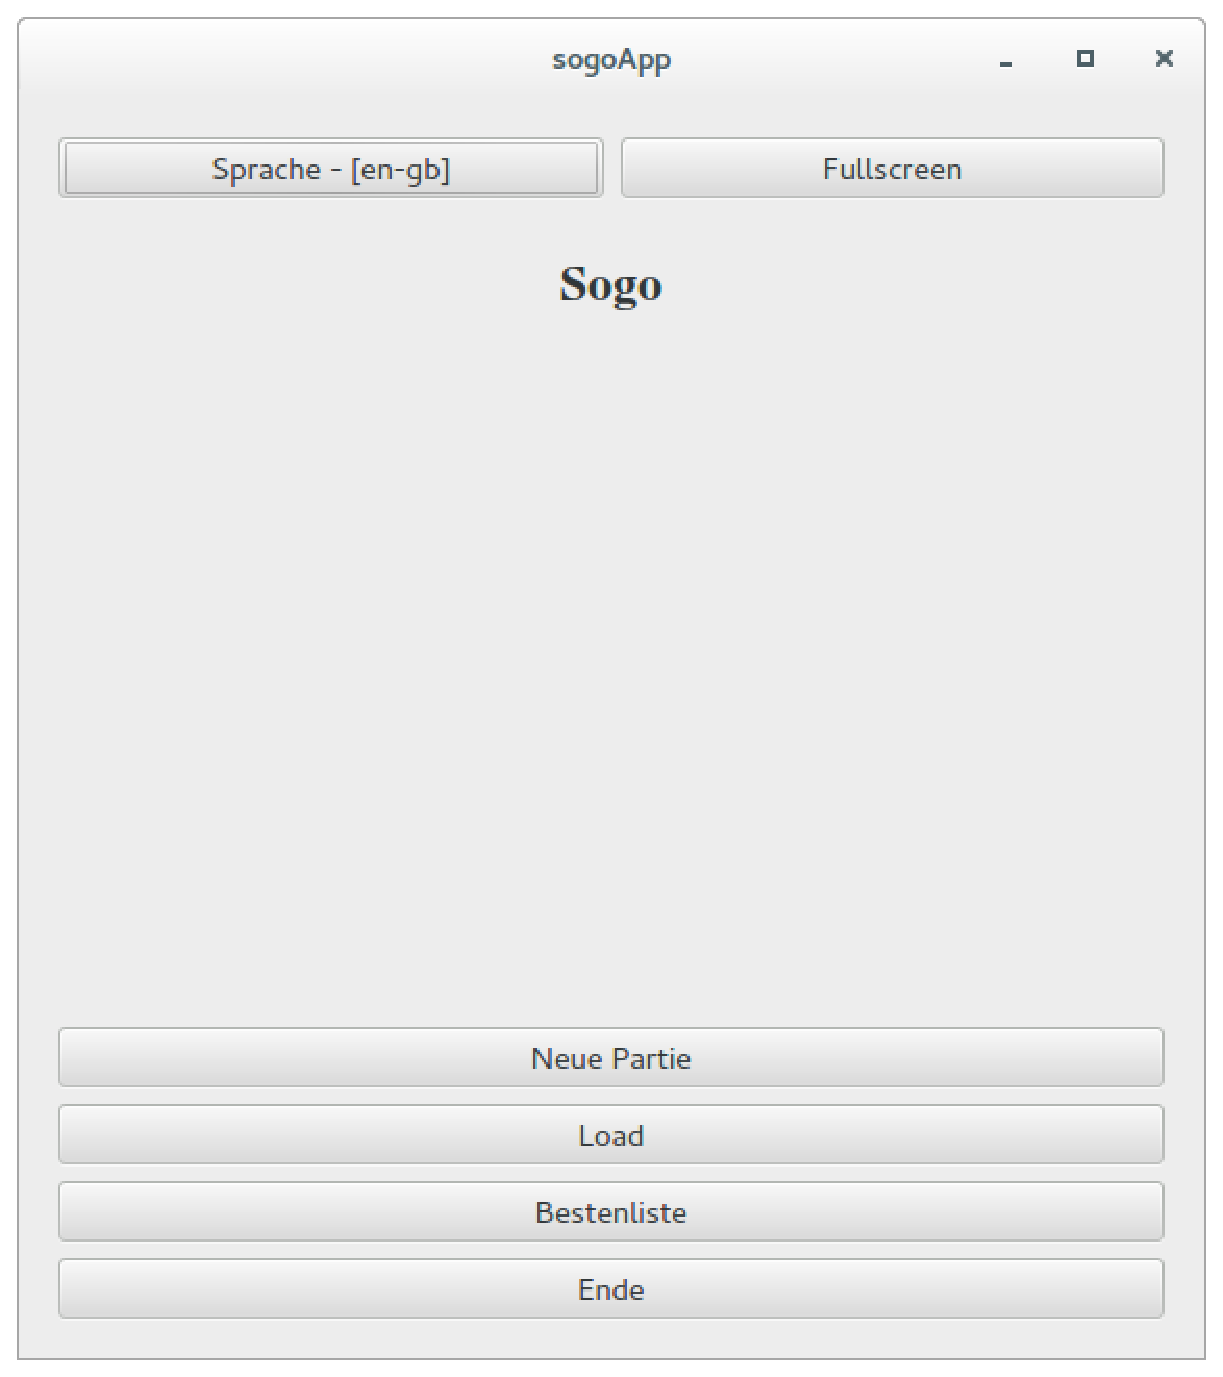
\includegraphics[scale=0.35]{graphics/startmenu.eps}
 \caption{Das Startmenü}
 \label{fig:Startmenü}
\end{figure}

\subsubsection{NewSessionMenu}\label{ch:NewSessionMenu}
Nachdem die Auswahl getroffen wurde ein neues Spiel zu beginnen, gelangt man in das NewSessionMenü, in dem die grundlegende Spielkonfiguration festgelegt werden kann. Die Konfigurationsmöglichkteiten werden durch die Abbildung~\ref{fig:NewSessionmenü} auf der Seite \pageref{fig:NewSessionmenü} dargestellt und im Folgenden kurz beschrieben. 

\begin{itemize}
	\item \textbf{Spieler1: } Hier kann der Name des ersten Spielers eingegeben werden, der wenn keiner eingegeben wird standardmäßig Spieler1 lautet.
	\item \textbf{Spieler1 beginnt: } Es wird festgelegt, dass der Spieler1 gebinnt.
	\item \textbf{Spielfeldgröße: } Hier wird die Spielfeldgröße festgelegt, welches im Standardspiel 4x4x4 ist.
	\item \textbf{Modus: } Über diese Option wird die Art des Spiels festgelegt. Wobei PvC für Player vs. Computer, PvP(lokal) für Player vs. Player am lokalen Rechner und PvP(Netzwerk) für Player vs. Player im Netzwerk steht. Wobei die Netzwerkkomponenten nicht implementiert wurde, was im Kapitel \ref{ch:Ergebnis} auf Seite \pageref{ch:Ergebnis} näher erläutert wird.
	\item \textbf{\glqq Schwierigkeitsgrad\grqq: } Sobald die Option PvC ausgewählt wurde, hat der Spieler die Möglichkeit den Schwierigkeitsgrad der KI auszuwählen. Dieser wird in den Stufen 1(leicht),2(mittel) und 3(schwer) angezeigt.  Durch jene Auswahl wird die Tiefe der Berechnung durch den MiniMax-Algorithmus aus dem Kapitel \ref{ch:AI} definiert. 
	\item \textbf{Spieler2: } Sobald die Option PvP ausgewählt wurde, kann im Textfeld der zweite Spielername eingetragen werden.
	\item \textbf{Spiel starten: } Das Spiel mit der momentan gesetzten Konfiguration starten.
	\item \textbf{Ende: } Damit wird die komplette Anwendung beendet.
\end{itemize}

Eine Besonderheit, die sich durch das ganze Projekt zog, war die Gestaltung des Frontends mittels Qt. Das soll heißen, dass jedes grafische Objekt verschachtelt und in ein Label, Widget und Layout verpackt wurde, was letztendlich dazu führte, dass die Anzahl der Attribute einer Klasse, an Komplexität zunahmen, wobei sich die Interaktionsmöglichkeiten  des Benutzers nur geringfügig veränderten.
 
\begin{figure}[H]
 \centering
 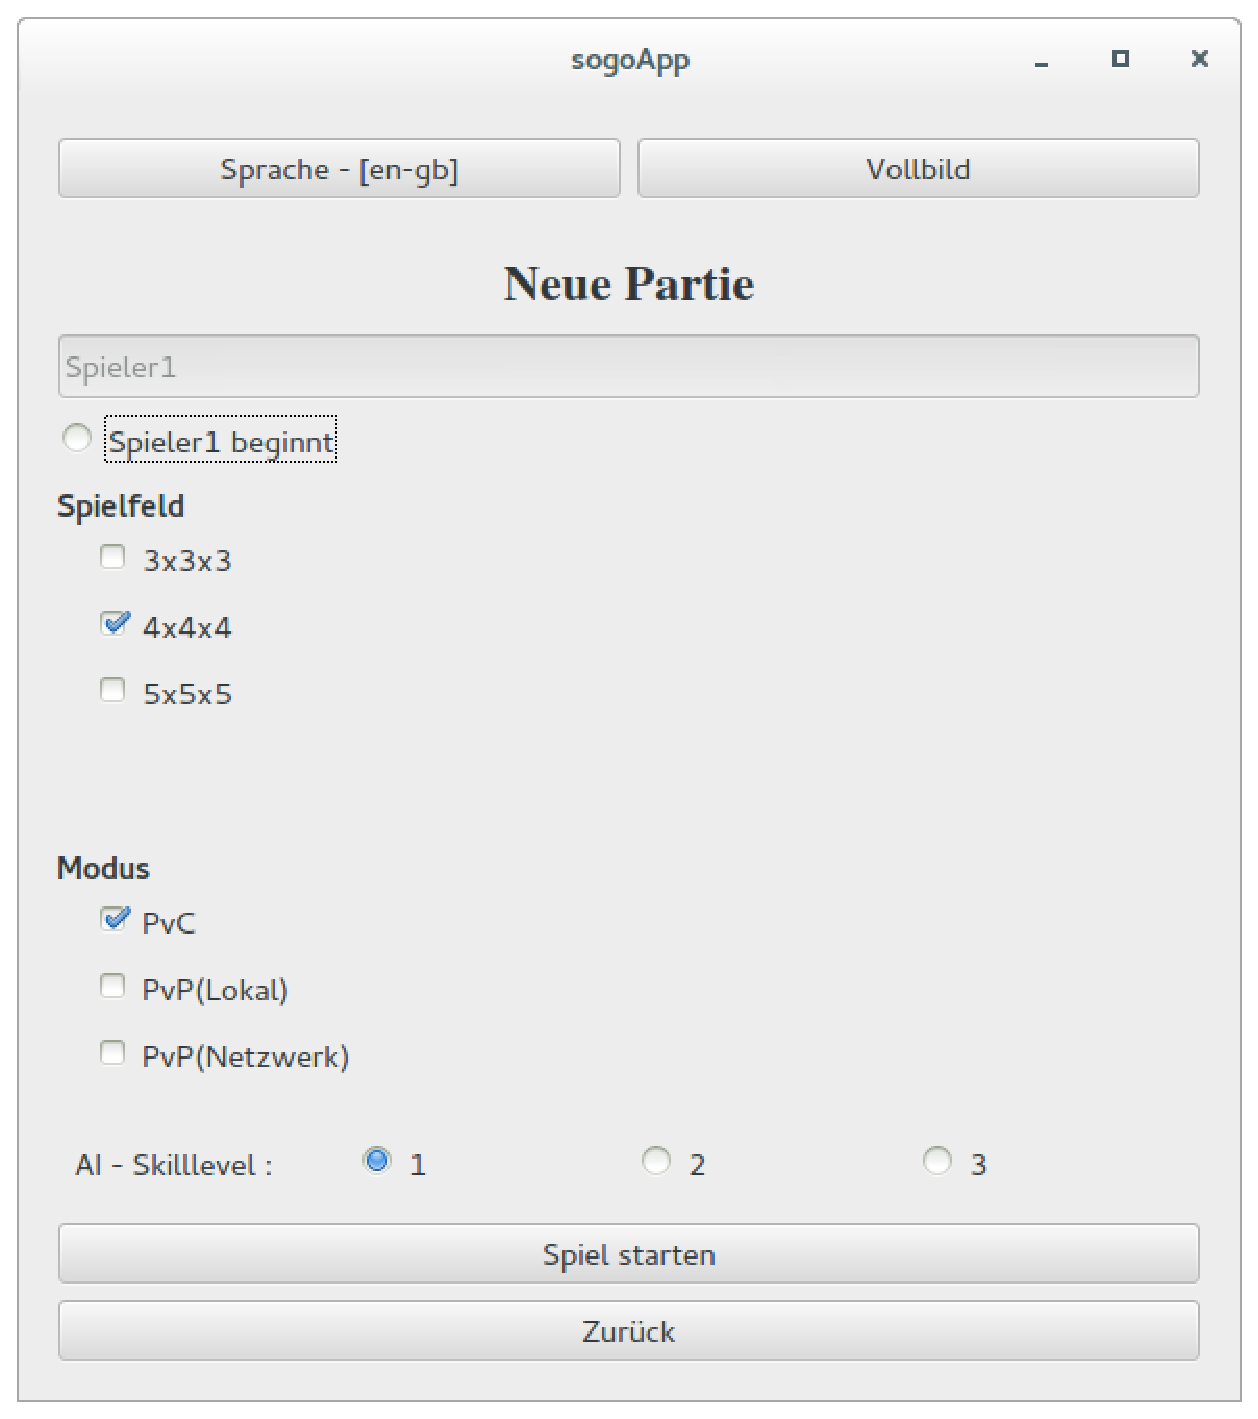
\includegraphics[scale=0.35]{graphics/newsession.eps}
 \caption{Das NewSessionmenü}
 \label{fig:NewSessionmenü}
\end{figure}

\subsubsection{HighscoreMenu}\label{ch:HighscoreMenu}
Dieses Menü dient der Anzeige, der einzelnen Partien und gibt sie entsprechend chronologisch der Spaltenbeschreibungen aus, wobei eine Partie, die mit einem Unentschieden endet, nicht mit aufgenommen wird.

\begin{figure}[H]
 	\centering
 	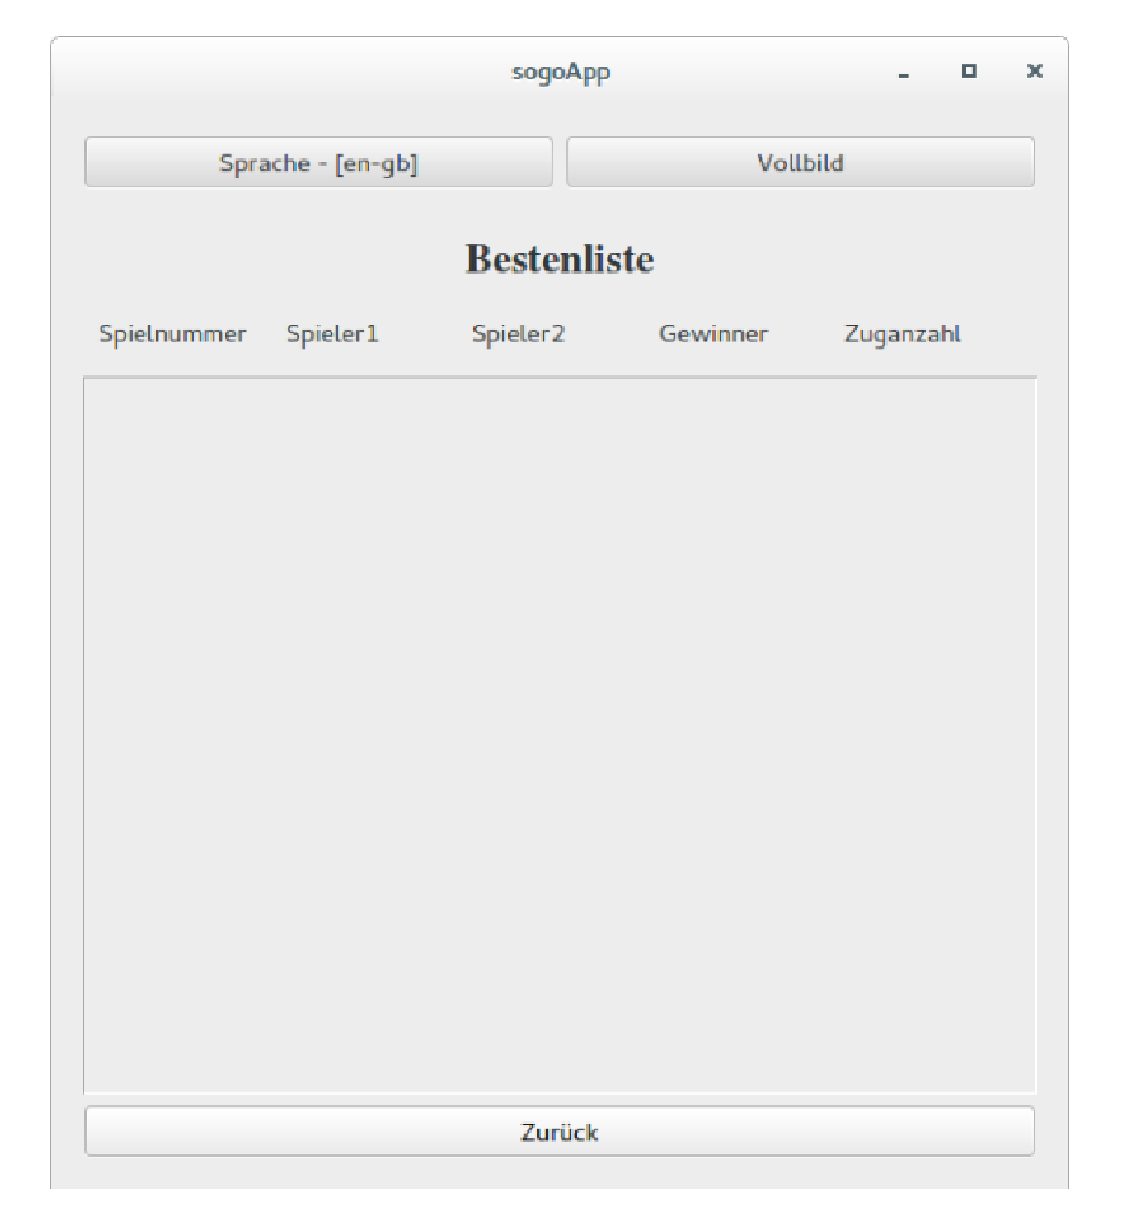
\includegraphics[scale=0.35]{graphics/highscore.eps}
 	\caption{Das Highscoremenü}
 	\label{fig:Highscoremenü}
\end{figure}

\subsubsection{PauseMenu}\label{ch:PauseMenu}
Durch diese Menü wollten wir eine Möglichkeit schaffen während einer Partie zu Pausieren oder sogar das Spiel zu beenden, um eventuell eine neue oder gespeicherte Partie zu starten.

\begin{figure}[H]
 \centering
 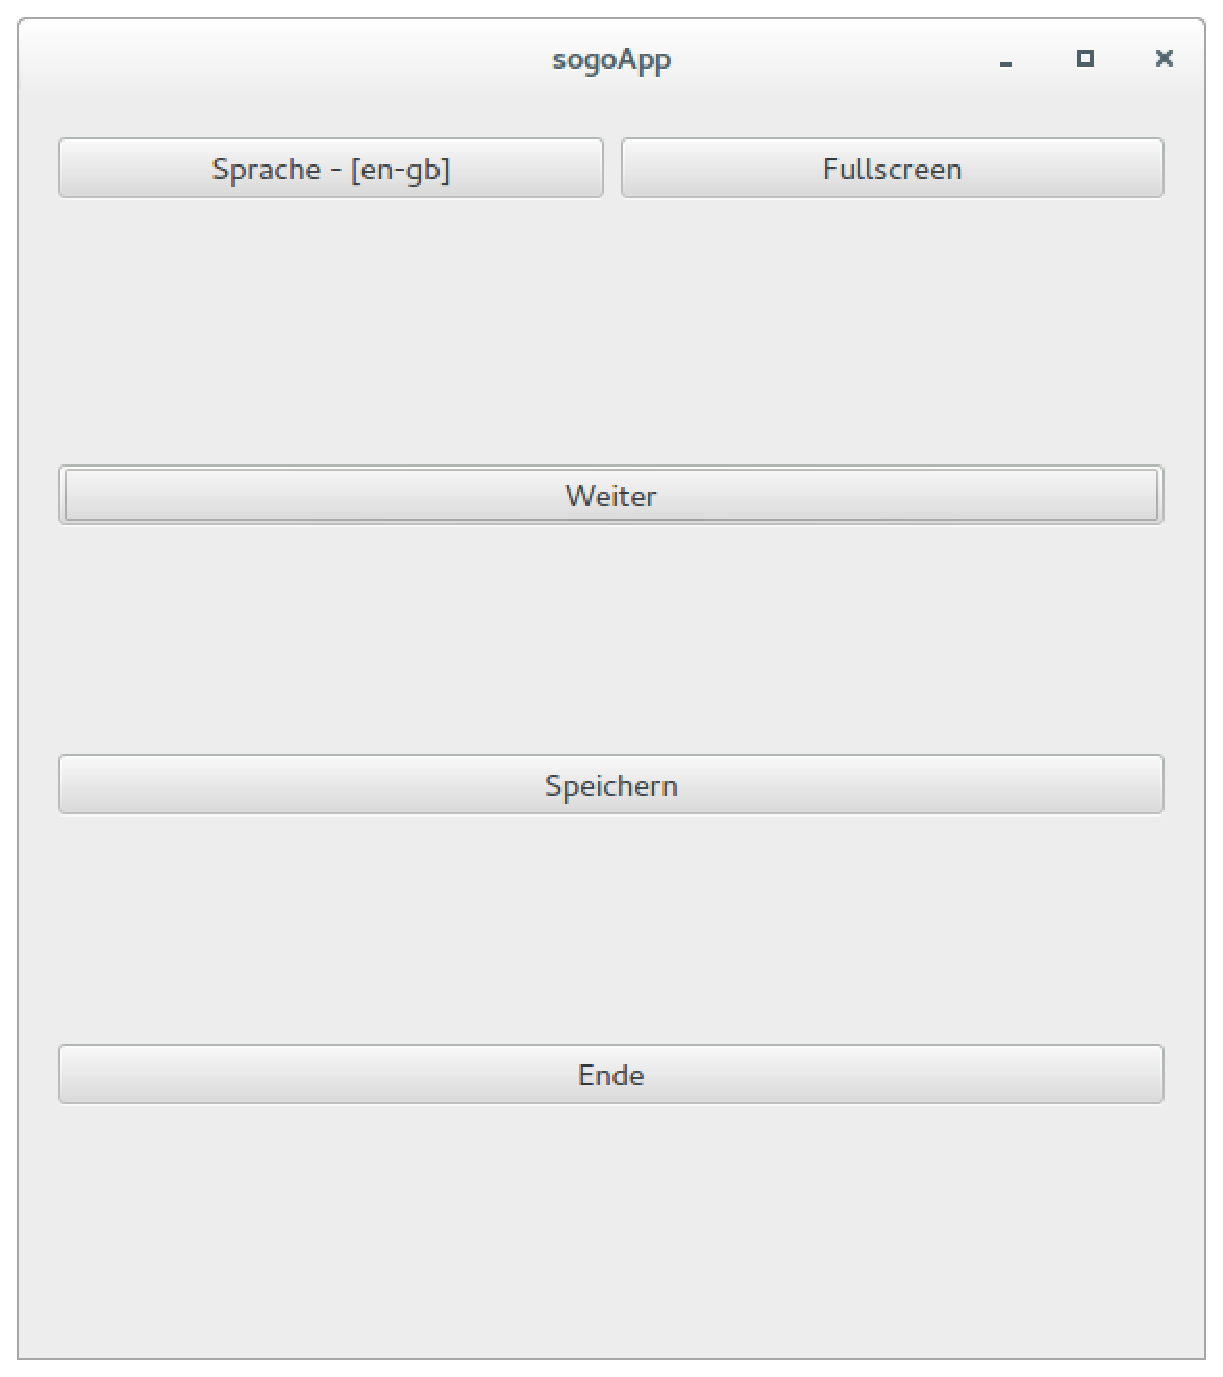
\includegraphics[scale=0.35]{graphics/pausemenu.eps}
 \caption{Das Pausemenü}
 \label{fig:Pausemenü}
\end{figure}

\subsubsection{Sprache}\label{ch:Sprache}
Ein Entscheidendes Kriterium war die Möglichkeit die Sprache zu jedem Zeitpunkt zu wechseln. Hierzu entschieden wir uns, die zwei, aus unserer Sicht, nützlichsten Sprachen zu wählen, nämlich deutsch und englisch. Dazu nutzten wir die Implementierung eines Translators. Hierzu wurden zwei erstellte .qm-Dateien den Ressourcen hinzugefügt, die die Übersetzung der einzelnen Textbausteine beinhalten. Um ein derartiges Wörterbuch zu erstellen, mussten sämtliche String-Texte, wie exemplarisch im Quellcodeausschnitt Quellcode~\ref{lst:Translatortext}: auf Seite \pageref{lst:Translatortext} dargestellt ist, formatiert werden. 

\begin{lstlisting}[caption={Translatortext}\label{lst:Translatortext},captionpos=t]
     m_playGameButton = new QPushButton(tr("Start Game"));
\end{lstlisting}
\textit{Die tr-Funktion gefolgt von dem Text, der übersetzt werden soll}
\\
\\
Damit eine Übersetzung einem Text zugeordnet werden kann, hat man die Möglichkeit die .gm-Dateien mittels Texteditor anzupassen oder den hauseigenen Translatoreditor Linguist von Qt zu verwenden, wobei die zweite Variante sehr komfortabel ist.
\\ 
\\
Damit innerhalb des Spiels die Sprache gewechselt werden kann, muss für jede Ansicht ein zusätzliches Event implementiert werden. Die Implementierungen werden in den folgenden Quelltextausschnitten dargestellt.

\begin{lstlisting}[caption={Translator}\label{lst:Translator},captionpos=t]
void MainWindow::ChangeLanguage()
{
    qApp->removeTranslator(m_translator);
    delete(m_translator);
    m_translator = new QTranslator();
    if(m_languageEnglish)
    {
        if(m_translator->load(":/sprache/Translations/sogoapp_de.qm"))
        {
            std::cout << "translator loaded" << std::endl;
        }
        else
        {
            std::cout << "translator did not load...whyever!!!" << std::endl;
        }
        m_languageEnglish = false;
    }
    else
    {
        if(m_translator->load(":/sprache/Translations/sogoapp_en.qm"))
        {
            std::cout << "translator loaded" << std::endl;
        }
        else
        {
            std::cout << "translator did not load...whyever!!!" << std::endl;
        }
        m_languageEnglish = true;
    }
    qApp->installTranslator(m_translator);

}
\end{lstlisting}
Hier werden die Sprachdateien geladen, die für die Übersetzung verantwortlich sind.

\begin{lstlisting}[caption={Sprachwechsel}\label{lst:Sprachwechsel},captionpos=t]
inline void changeEvent(QEvent *event)
    {
        if (event->type() == QEvent::LanguageChange) {
            m_newSessionButton->setText(tr("New Session"));
            m_highscoreButton->setText(tr(("Highscore")));
            m_exitButton->setText(tr("Exit"));

        } else
            QWidget::changeEvent(event);
    }
\end{lstlisting}
Anschließend wurde der Sprachwechsel mit einen Button im Frontend verknüpft und auf jeder Ansicht zugänglich gemacht.

\subsection{Mainwindow}\label{ch:Mainwindow}
Das Mainwindow beinhaltet die komplette Implementierung, samt Spiellogik, 2D- und 3D- Bereich sowie das Frontend der Sogo-Applikation. Sie ist es letztendlich, die in der Main-Funktion deklariert und initialisiert wird. Außerdem werden hier Signale die von Inputs oder Spielereignissen aufgerufen werden mit entsprechenden Screen- oder Spielbestandteilsignalen verknüpft.

\subsection{GameView}\label{ch:GameView}
Hier wird die Darstellung des aktuellen Spiels mit 2D- und 3D-View, Spielverlaufsanzeige und Spielereingabe verwaltet.

\subsubsection{GameView2D}\label{ch:GameView2D}
Die GameView2D Datei enthält die Implementierung des 2D Displays. Es zeigt die Ebenen des Spielfeldes nebeneinander in QGraphicsViews an. In diesen QGraphicsViews werden die GraphicsSlots2D gezeichnet, welche als ein Quadrat dargestellt und mit der Farbe der Belegung befüllt werden. Die Farbbelegung sieht wir folgt aus
\begin{itemize}
	\item weiß für Freifläche
	\item blau für Spieler1
	\item rot für Spieler2
\end{itemize}

\subsubsection{GameView3D}\label{ch:GameView3D}
Die GameView3D Datei enthält die Implementierung des 3D Displays. In der initializeGL Methode werden Texturen, 3D-Modelle und die OpenGL Einstellungen initialisiert. In der paintGL wird der aktuelle Zustand des Spielfeldes
in 3D umgesetzt, dabei wird, wie bei der 2D Umsetzung, auch das Feld Slot für Slot durchgegangen und je nach Belegung wird entweder ein leerer Stab, eine blaue oder eine rote Kugel gezeichnet. Die Darstellungen des Spielfeldes wird 30 mal pro Sekunde komplett neu generiert. Der View ist interaktiv, insofern, dass man in mit den W-A-S-D-Tasten drehen und mit der Maus die Spielsteine setzen kann. Einen Eindruck davon erhält man, wenn man die unten stehende Abbildung betrachtet.

\begin{figure}[H]
 \centering
 \includegraphics[scale=0.65]{graphics/3dView.eps}
 \caption{Die 3D-Ansicht}
 \label{fig:3dVuew}
\end{figure} 

\subsection{Logger - Der hauseigene Debugger}\label{ch:Logger}
Dieses kleine Stück Quelltext, siehe unten stehenden Quellcode~\ref{lst:CodeLogger}: auf Seite \pageref{lst:CodeLogger}, welches uns dabei geholfen hat den Großteil der aufgetretenen Fehler ausfindig zu machen und zu beheben. Durch die zunehmende Komplexität des Projektes und der damit verbundenen Zunamen an Quelltext haben wir, eine Möglichkeit geschaffen, den Quelltext in einzelne Abschnitte zu unterteilen und sie auf ihre Funktion zu überprüfen, um dadurch die Fehlerquelle ausschließen zu können. Dieses Stück Quelltext ist, in unseren Augen, ein ideales Beispiel für das Wiederverwenden von Quelltext in zukünftigen Projekten, wobei eine kontinuierliche Weiterentwicklung angestrebt werden sollte.
\lstinputlisting
    [caption={Logger - Debugger} 	% Titel
    	\label{lst:CodeLogger},			% Zum Referenzieren    
    emptylines=0,					% Zulassen der leeren Zeilen.(hier keine)
    captionpos=t,					% Titelanzeige on top(t)
    language=c++,					% Programmiersprache
    linerange={19-26,33-40,48-55,62-69,79-86}]%,98-110}]	% Auswahl Zeilen
{../../src/utility/Logger.cpp}		% Sourcefile
%external
\subsection{3D Umsetzung}\label{ch:3DUmsetzung}
Die 3D-Umsetzung stellte wohl den größten und gleichzeitig kompliziertesten Teil des Projektes dar. Wie im Kapitel~\ref{ch:Analyse} beschrieben, haben wir einen enormen Aufwand betrieben, um diesen zu implementieren, obwohl er nur einen relativ kleinen Anteil zum Gesamtprojekt darstellt. Unsere Zeitkalkulation sah diesen Aufwand in diesem Ausmaß nicht vor, welches wir nicht vorhersehen konnten. Unserer Auffassung nach, hätten wir den bereits erstellten Quelltext im Fach Computergrafik, fast vollständig in Qt überführen können inklusive der Anpassung an die Qt-Syntax, da Qt die Nutzung von OpenGL unterstützt. 

% /===========================================================================\
%   Test
% \===========================================================================/
\section{Test}\label{ch:Test}
\subsection{Unit-Test}\label{ch:Unit}
Schon zu Beginn des Projektes haben wir uns recht früh mit dem Thema Unit-Test auseinandergesetzt. Doch letztendlich wurden sie nur in der Konsolen-Applikation realisiert. Diese Tests sollten die Spielweise der KI als auch die 
Funktionsweise des Spielfeldes testen, was sie letztendlich auch tun. Diese Konsolen-Version stellt unseren Prototypen dar, was zur Folge hatte, dass die Unit-Test die bereits erfolgreich liefen, nicht in die eigentliche Applikation überführt und implementiert wurden. Sie befinden sich im Verzeichnis tests. Im Nachhinein betrachtet, war dies eine vertane Möglichkeit sich einen kontinuierlichen Workflow anzueignen. Nichtsdestotrotz haben wir kontinuierliche und ausführliche Playtest durchgeführt, die die Funktionalität bestätigten.

\subsection{Valgrind - Docker}\label{ch:Valgrind&Docker}
Um Valgring einzusetzen war es notwendig den Quelltext mittels qmake/make zu kompilieren und anschließend auszuführen. Doch diser Schritt war nicht möglich, da die 3D-Komponente Fehler verursachte, die bis zum Abgabetermin nicht behoben werden konnten. Also haben wir versucht den Memcheck mittels Valgrind im Qt Creator durchzuführen, was dazu führte, dass dieser sich nicht mehr beendete und damit keine Ergebnisse ausgeben konnte.
\\
Ebenso war es uns nicht möglich auf Grund des 3D-Views die Containerlösung zu realisieren. Letztendlich war die Zeitintensive implementierung der 3D-Komponente ausschlaggebend für Umsetzung der zum Teil noch fehlenden Anforderungen aus dem Kapitel~\ref{ch:Test}.

\subsubsection{Sounds}\label{ch:Sounds}
Die Verwendeten Sounds stammen vom Unity-Asset Store.

% /===========================================================================\
%   Ergebnis
% \===========================================================================/
\section{Ergebnis}\label{ch:Ergebnis}
\subsection{Soll-Ist-Vergleich}\label{ch:Vergleich}
Auf Grundlagen der zu Beginn des Projektes verfassten Anforderungen wollen wird nur jene aufzeigen, die nicht in unser Projekt eingeflossen sind und erklären warum diese nicht implementiert wurden. Doch bevor wir damit beginnen, wollen wir auf die Anforderung eingehen, die letztendlich realisiert, weit über das vorgegebenen Zeitkontingent hinausgeschossen ist und die damit einen großen Einfluss auf die bisher realisierten als auch nicht realisierten Anforderungen hatte. Die 3D-Ansicht. Die Besonderheit war, dass es gleichzeitig die Belegarbeit im Fach Computergrafik darstellte. Somit musste diese Anforderung realisiert werden. Letztendlich auf Kosten von Anforderungen, die nicht umgesetzt wurden. Im Verlauf des Projektes(Semesters) war Herr Brandt in der Lage einen Prototypen, in Form einer Konsolenanwendung, zu realisieren, der die grundlegenden Funktionen beinhaltete und auf dem die gegenwärtige Applikation aufgebaut. Zur gleichen Zeit beendete Professor Jung, im Fach Computergrafik, seinen sog. Pflichtteil, der die Grundlage für unsere 3D-Ansicht darstellt. Mit diesem Wissen erstellten wir in Visual Studio 2015 und der grafischen Bibliothek OpenGL Sogo in 3D als reine Visualisierungsmöglichkeit. Die eigentliche Arbeit folgte danach. Die Überführung und Anpassung des Quelltextes aus Visual Studio nach Qt und Integration der Spiellogik. Einer der Gründe weswegen die Überführung so schwierig war, waren die nur spärlich vorhandenen Referenzprojekte sowie die oberflächliche Dokumentation von Qt im Bereich OpenGL. Letztendlich stellten wir uns nach der Hälfte der vorgegebenen Zeit die Frage, ob und wie wir die Projekte in beiden Fächern realisieren konnten. Die erste Alternative war die Projekte wieder aufzuspalten und in der jeweiligen Umgebung zu realisieren. Das hätte bedeutet, dass die 3D-Ansicht mittels Visual Studio 2015 umgesetzt hätte werden müssen und die 2D-Variante ohne 3D in Qt. Die Konsequenz daraus wäre gewesen, dass die komplette Spiellogik redundant in beiden Applikationen hätte realisiert werden müssen. 
Die zweite Alternative war die Kombination aus der Ersten mit der Überlegung das Projekt noch eine Woche weiterzuführen wie bisher. Das bedeutete, sollte es uns nicht gelingen, würden wir beide Projekte getrennt von einander entwickeln und abgeben. Wir entschieden uns für die zweite Alternative und schafften es die Überführung des Quelltextes ohne Fehler am letzten Tag der Frist zu implementieren. Was danach folgte war die Anpassung an die Spiellogik, welche sich ebenfalls weiterentwickelt hatte, und die Modifizierung der grafischen Oberfläche. Die Zeit, die wir investierten fehlte uns im Nachhinein bei Umsetzung einiger der folgenden Anforderungen. Beginnen wollen wir mit den projektunabhängigen Anforderungen:
\\
\\
\textbf{Anforderung:} Die Applikation läuft auf einem Desktop-Rechner, wird aber auch auf einer mobilen Plattform getestet und wenn nötig angepasst.
\\
\textbf{Beschreibung:}  Sie läuft auf einem Desktop-Rechner und wurde aus o.g. Zeitgründen bisher noch nicht auf mobilen Plattformen getestet. 
\\
\\
\textbf{Anforderungen an den Enwicklungsprozess:}
\\
\\
\textbf{Anforderung:} Fehlerfreies Belegen der Implementierung der Datenstrukturen und Algorithmen durch Unit-Tests. 
\\
\textbf{Beschreibung:} Dies wurde bereits im Kapitel~\ref{ch:Unit}: auf Seite \pageref{ch:Unit} näher erläutert.

% valgrind
% docker

\textbf{Eigene Anforderungen:}
\\
\\
\textbf{Anforderung:} Die Spielstände sollen in einer lokalen SQL-DB gespeichert werden.
\\
\textbf{Beschreibung:} Die Spielständer werden in einer einzelnen Datei gespeichert und dienen dem Highscore als Grundlage.
\\
\\
\textbf{Anforderung:} (Zusammenfassung) Die Möglichkeit das Spiel über das Netzwerk zu spielen inklusive Chatfunktion.
\\
\textbf{Beschreibung:} Auf Grund der o.g. Problematik bezüglich der 3D-Ansicht, sind die Anforderungen der des Netzwerkspiels entfallen. Es existiert die Möglichkeit alle notwendigen Daten in eine Maske einzutragen, jedoch ist diese nicht mit einer Funkion hinterlegt.
\\
\\
\textbf{Anforderung:} Das Zurücknehmen eines getätigten Zuges. 
\\
\textbf{Beschreibung:} Wurde aus Zeitgründen nicht realisiert.
\\
\\
\textbf{Anforderung:} Die Besonderheit beim Spielen mit der Feldgröße 5x5x5 (setzen von unten).
\\
\textbf{Beschreibung:} Aus Zeitgründen wurde die Standardlogik verwendet und implementiert. Hinzukommt, dass die Komplexität der Implementierung für die 3D-Umsetzung noch weiter erhöht hätte.

\subsection{Bewertung - Fazit}\label{ch:Bewertung}
Diese Projekt stellte, wie bereits zu beginn des Semester dargelegt, das umfangreichste Softwareprojekt dar, welches als Beleg abzugeben war bzw. ist. Jedoch konnte man dadurch seine Kenntnisse im Bereich der C++-Programmierung und des Projektmanagement weiter festigen und vertiefen. Die größte Hürde war aus unserer Sicht den richtigen Einstieg zu finden, da Vorlesungsinhalte, die zur Realisierung benötigt wurden, erst recht spät oder gar nicht im Semester behandelt wurden siehe Mini-Max-Algorithmus. Für unser spezielles Projekt wäre es sinnvoll gewesen eine komplette Vorlesungseinheit Qt in Verbindung mit OpenGL durchzuführen, wobei uns auch klar ist, dass aus zeitlichen Gründen nicht alle Aspekte angesprochen werden können. Wie im Kapitel~\ref{ch:Ergebnis} beschrieben, haben wir die Thematik Valgrind, Docker und Unit-Test nur teilweise umgesetzt. Die Gründe haben wir bereits dargelegt, jedoch wollen wir noch mal festhalten, dass wir für zukünftige Projekte dieser Techniken einfließen lassen wollen, da sie eine weitere Möglichkeit darstellen zum einen den Quelltext zu überprüfen und zum Andern die Applikation modular einzusetzen. Durch dieses Projekt hat man einen kleinen Einblick in die Erstellung von kooperativen Softwareprojekten bekommen und welche Schwierigkeiten dabei auftreten können. Die gewonnenen Kenntnisse werden helfen um zukünftige Softwareprojekte besser zu planen, durchzuführen und erfolgreich abzuschließen. 

\subsection{Ausblick}\label{ch:Ausblick}
Natürlich wäre es schön, wenn diese Applikation durch die noch fehlenden Anforderungen vervollständigt werden würde. Sowie es vorstellbar wäre das Frontend anzupassen um es an die Optik des Spiels anzupassen. Die Grundlage dafür wurde durch die Verwendung von Github und des frei zugänglichen Repositorie\cite{GitRepo16} geschaffen. Aus unserer Sicht werden definitiv Teile der Applikation in Folgeprojekte verwendet und weiterentwickelt, sowie bspw. der Logger aus Kapitel~\ref{ch:Logger} oder der KI aus dem Kapitel~\ref{ch:3DUmsetzung}.

\newpage

% 
% /===========================================================================\
%
% 	Literaturverzeichnis
%
% \===========================================================================/
\printbibliography 

\addcontentsline{toc}{section}{Literaturverzeichnis}	% Anzeige im Inhaltsverzeichnis(table of content [toc]) als Abschnitt[section] unter dem Titel[Literaturverzeichnis]

\newpage

% /===========================================================================\
%
% 	Abbildungsverzeichnis
%
% \===========================================================================/
\listoffigures

\addcontentsline{toc}{section}{Abbildungsverzeichnis}	% Anzeige im Inhaltsverzeichnis

\newpage

% /===========================================================================\
%
% 	Quellcodeverzeichnis
%
% \===========================================================================/
\renewcommand{\lstlistlistingname}{Quellcodeverzeichnis}	% Setzt den Titel des Quellcodeverzeichnis von Listings auf Quelcodeverzeichnis

\lstlistoflistings 

\addcontentsline{toc}{section}{Quellcodeverzeichnis}	% Anzeige im Inhaltsverzeichnis

\newpage

\end{document}